
\documentclass[11pt]{article}
\usepackage[margin=0.75in]{geometry}
\usepackage{booktabs}
\usepackage{array}
\usepackage{longtable}
\usepackage{graphicx}
\usepackage{xcolor}
\usepackage{hyperref}
\usepackage{pgfplots}
\usepackage{pgfplotstable}
\usepackage{float}
\pgfplotsset{compat=1.18}
\hypersetup{colorlinks=true, linkcolor=blue, urlcolor=blue}
\definecolor{cblue}{HTML}{1F77B4}
\definecolor{corange}{HTML}{FF7F0E}
\definecolor{cgreen}{HTML}{2CA02C}
\definecolor{cred}{HTML}{D62728}
\definecolor{cpurple}{HTML}{9467BD}
\definecolor{cgray}{HTML}{666666}
\setlength{\parskip}{0.45em}
\setlength{\parindent}{0pt}

\title{Motif Statistics in Optimized Inventory Policies}
\author{DeepSeek + SciPy EoH Runs}
\date{May 2026}

\begin{document}
\maketitle

\begin{abstract}
This report summarizes structural motifs in optimized inventory-control policies. The analysis uses a conservative static detector applied to saved population files, focusing on high-coverage DeepSeek+SciPy runs. The main finding is that policies retain an order-up-to/base-stock backbone while increasingly adding partial adjustment, pipeline weighting, and order clipping across generations. Distribution families show different dominant refinements: exponential instances emphasize smoothing and pipeline timing, Poisson instances emphasize clipping, and normal instances retain the strongest order-up-to structure.
\end{abstract}

\section{Scope and Data}
The analysis uses policies from \texttt{pops/population\_generation\_*.json}, not prompt files, because these files provide explicit generation identifiers. The scope is:
\begin{itemize}
  \item Model and optimizer: DeepSeek + SciPy, operator \texttt{m2}.
  \item Generations: 1 through 10.
  \item Distributions: the 14 distributions whose prompt-cost matching rate exceeded 80\% under the previous 1\% same-distribution matching rule.
  \item Sample size: 5,052 policy records from 53 run folders.
\end{itemize}

\section{Conservative Motif Detector}
The detector uses Python AST parsing and dependency tracking from the final order expression. It is intentionally conservative:
\begin{itemize}
  \item \textbf{Inventory position} requires an unweighted combined signal using on-hand inventory and total pipeline inventory.
  \item \textbf{Order-up-to} requires a positive-part target-minus-state gap, such as \texttt{max(0, target - state)}.
  \item \textbf{Partial adjustment} requires a gain or smoothing parameter multiplying a gap/order response.
  \item \textbf{Pipeline weighting} requires weighted pipeline terms on the dependency path to the final order decision.
  \item \textbf{Constant order} requires an additive baseline in the final order expression, not merely safety stock inside a target level.
  \item \textbf{Order clipping} detects upper/lower bounding beyond the positive-part operator.
  \item \textbf{Thresholding} requires a meaningful state/order threshold that controls the order formula, excluding implementation checks such as \texttt{len(pipeline\_orders)>0}.
\end{itemize}

\section{Overall Motif Frequencies}
Average number of motifs per policy: \textbf{3.43}.

\begin{table}[H]
\centering
\caption{Overall motif frequencies}
\begin{tabular}{lr}
\toprule
Motif & Frequency \\
\midrule
Inventory position & 81.6\% \\
Order-up-to & 87.1\% \\
Partial adjustment & 55.1\% \\
Pipeline weighting & 43.5\% \\
Constant order & 14.4\% \\
Order clipping & 52.7\% \\
Thresholding & 9.0\% \\
\bottomrule
\end{tabular}
\end{table}

\textbf{Interpretation.} The order-up-to motif remains the dominant backbone. However, more than half of the policies include partial adjustment or clipping, and roughly 43\% use some form of pipeline weighting. This indicates that optimization does not simply replace base-stock logic; it layers control refinements on top of a target-seeking structure.

\section{Generation-Wise Pattern}

\begin{figure}[H]
\centering
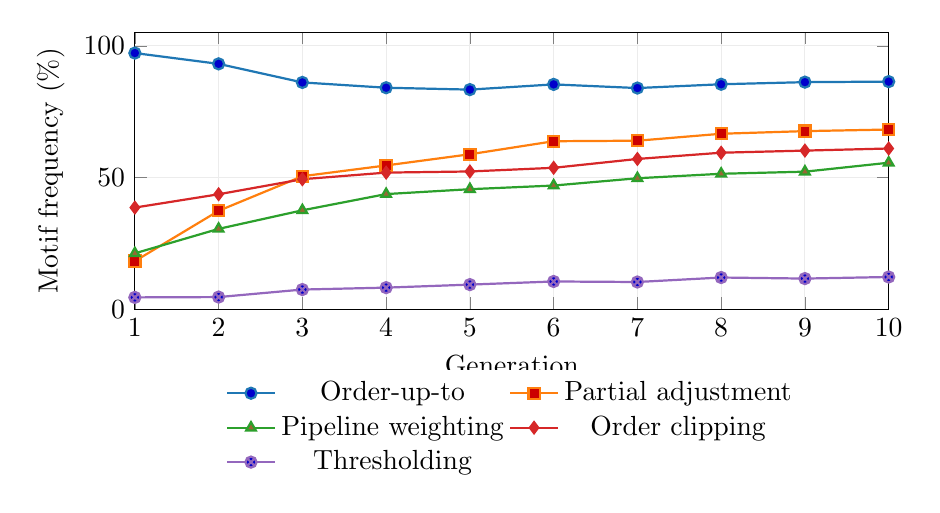
\begin{tikzpicture}
\begin{axis}[
    width=0.92\textwidth,
    height=0.42\textwidth,
    xlabel={Generation},
    ylabel={Motif frequency (\%)},
    xmin=1, xmax=10,
    ymin=0, ymax=105,
    xtick={1,2,3,4,5,6,7,8,9,10},
    legend columns=2,
    legend style={at={(0.5,-0.22)},anchor=north,draw=none},
    grid=both,
    grid style={gray!15},
]
\addplot+[mark=*, color=cblue, thick] coordinates {(1,97.2458) (2,93.1429) (3,86.0952) (4,84.0777) (5,83.3663) (6,85.3465) (7,83.9604) (8,85.4000) (9,86.2000) (10,86.4000)}; \addlegendentry{Order-up-to}
\addplot+[mark=square*, color=corange, thick] coordinates {(1,18.2203) (2,37.3333) (3,50.4762) (4,54.5631) (5,58.8119) (6,63.7624) (7,63.9604) (8,66.6000) (9,67.6000) (10,68.2000)}; \addlegendentry{Partial adjustment}
\addplot+[mark=triangle*, color=cgreen, thick] coordinates {(1,21.1864) (2,30.4762) (3,37.5238) (4,43.6893) (5,45.5446) (6,46.9307) (7,49.7030) (8,51.4000) (9,52.2000) (10,55.6000)}; \addlegendentry{Pipeline weighting}
\addplot+[mark=diamond*, color=cred, thick] coordinates {(1,38.5593) (2,43.6190) (3,49.3333) (4,51.8447) (5,52.2772) (6,53.6634) (7,57.0297) (8,59.4000) (9,60.2000) (10,61.0000)}; \addlegendentry{Order clipping}
\addplot+[mark=otimes*, color=cpurple, thick] coordinates {(1,4.4492) (2,4.5714) (3,7.4286) (4,8.1553) (5,9.3069) (6,10.4950) (7,10.2970) (8,12.0000) (9,11.6000) (10,12.2000)}; \addlegendentry{Thresholding}
\end{axis}
\end{tikzpicture}
\caption{Motif frequencies by generation.}
\end{figure}

\begin{figure}[H]
\centering
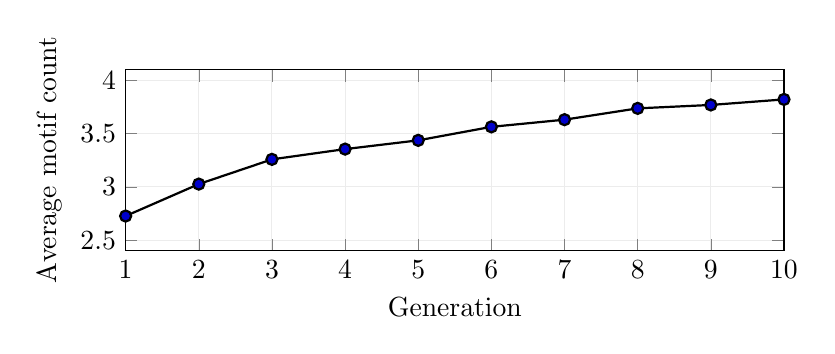
\begin{tikzpicture}
\begin{axis}[
    width=0.82\textwidth,
    height=0.32\textwidth,
    xlabel={Generation},
    ylabel={Average motif count},
    xmin=1, xmax=10,
    ymin=2.4, ymax=4.1,
    xtick={1,2,3,4,5,6,7,8,9,10},
    grid=both,
    grid style={gray!15},
]
\addplot+[mark=*, color=black, thick] coordinates {(1,2.7267) (2,3.0267) (3,3.2590) (4,3.3553) (5,3.4376) (6,3.5644) (7,3.6317) (8,3.7380) (9,3.7700) (10,3.8220)};
\end{axis}
\end{tikzpicture}
\caption{Average number of detected motifs per policy.}
\end{figure}

\begin{table}[H]
\centering
\caption{Selected generation-wise statistics}
\small
\begin{tabular}{rrrrrrrr}
\toprule
Gen & N & Avg. motifs & Order-up-to & Partial & Pipeline & Clipping & Threshold \\
\midrule
1 & 472 & 2.73 & 97.2 & 18.2 & 21.2 & 38.6 & 4.4 \\
2 & 525 & 3.03 & 93.1 & 37.3 & 30.5 & 43.6 & 4.6 \\
3 & 525 & 3.26 & 86.1 & 50.5 & 37.5 & 49.3 & 7.4 \\
4 & 515 & 3.36 & 84.1 & 54.6 & 43.7 & 51.8 & 8.2 \\
5 & 505 & 3.44 & 83.4 & 58.8 & 45.5 & 52.3 & 9.3 \\
6 & 505 & 3.56 & 85.3 & 63.8 & 46.9 & 53.7 & 10.5 \\
7 & 505 & 3.63 & 84.0 & 64.0 & 49.7 & 57.0 & 10.3 \\
8 & 500 & 3.74 & 85.4 & 66.6 & 51.4 & 59.4 & 12.0 \\
9 & 500 & 3.77 & 86.2 & 67.6 & 52.2 & 60.2 & 11.6 \\
10 & 500 & 3.82 & 86.4 & 68.2 & 55.6 & 61.0 & 12.2 \\
\bottomrule
\end{tabular}
\end{table}

From generation 1 to generation 10, average motif count increases from 2.73 to 3.82. The largest changes are:
\begin{itemize}
  \item Partial adjustment: +50.0 percentage points.
  \item Pipeline weighting: +34.4 percentage points.
  \item Order clipping: +22.4 percentage points.
  \item Thresholding: +7.8 percentage points.
\end{itemize}

\begin{table}[H]
\centering
\caption{Motif-count distribution in generation 1 vs. generation 10}
\begin{tabular}{rrr}
\toprule
Number of motifs & Gen. 1 share (\%) & Gen. 10 share (\%) \\
\midrule
0 & 0.0 & 0.0 \\
1 & 1.3 & 1.2 \\
2 & 44.5 & 10.8 \\
3 & 38.8 & 28.6 \\
4 & 11.4 & 29.2 \\
5 & 3.8 & 24.4 \\
6 & 0.2 & 5.8 \\
7 & 0.0 & 0.0 \\
\bottomrule
\end{tabular}
\end{table}

\textbf{Takeaway.} Early policies are mostly simple 2--3 motif rules. By generation 10, mass shifts toward 4--6 motif policies, consistent with progressive structural enrichment.

\section{Distribution-Wise Differences}

\begin{table}[H]
\centering
\caption{Family-level weighted averages}
\small
\begin{tabular}{lrrrrrrr}
\toprule
Family & N & Avg. motifs & Order-up-to & Partial & Pipeline & Clipping & Threshold \\
\midrule
Exponential & 1431 & 3.63 & 87.9 & 64.1 & 56.0 & 45.2 & 7.8 \\
Poisson & 3124 & 3.34 & 84.7 & 52.6 & 37.7 & 54.8 & 8.8 \\
Normal & 497 & 3.46 & 99.4 & 44.7 & 43.7 & 61.4 & 14.3 \\
\bottomrule
\end{tabular}
\end{table}

\begin{figure}[H]
\centering
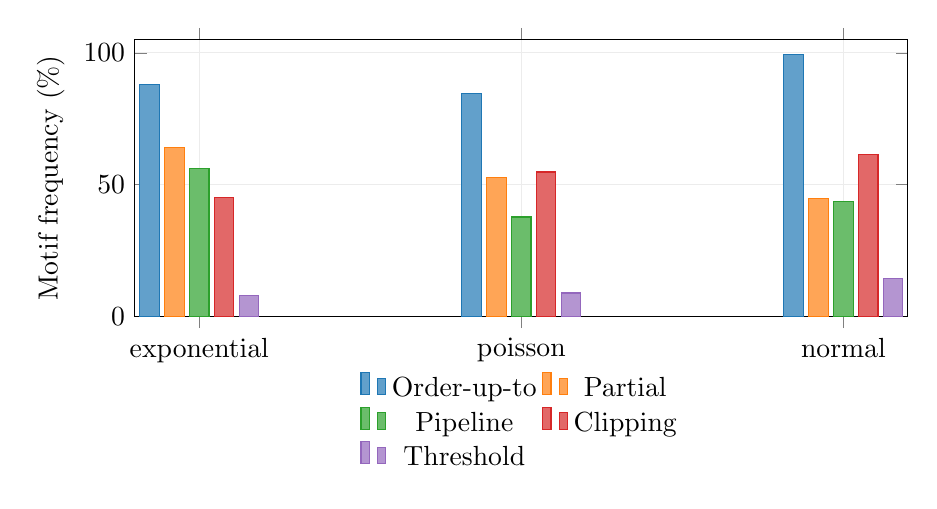
\begin{tikzpicture}
\begin{axis}[
    ybar,
    bar width=7pt,
    width=0.94\textwidth,
    height=0.42\textwidth,
    ylabel={Motif frequency (\%)},
    symbolic x coords={exponential,poisson,normal},
    xtick=data,
    ymin=0, ymax=105,
    legend columns=2,
    legend style={at={(0.5,-0.18)},anchor=north,draw=none},
    grid=major,
    grid style={gray!15},
]
\addplot+[fill=cblue!70, draw=cblue] coordinates {(exponential,87.9105) (poisson,84.7311) (normal,99.3964)}; \addlegendentry{Order-up-to}
\addplot+[fill=corange!70, draw=corange] coordinates {(exponential,64.0811) (poisson,52.5928) (normal,44.6680)}; \addlegendentry{Partial}
\addplot+[fill=cgreen!70, draw=cgreen] coordinates {(exponential,56.0447) (poisson,37.6761) (normal,43.6620)}; \addlegendentry{Pipeline}
\addplot+[fill=cred!70, draw=cred] coordinates {(exponential,45.2131) (poisson,54.7695) (normal,61.3682)}; \addlegendentry{Clipping}
\addplot+[fill=cpurple!70, draw=cpurple] coordinates {(exponential,7.7568) (poisson,8.8028) (normal,14.2858)}; \addlegendentry{Threshold}
\end{axis}
\end{tikzpicture}
\caption{Motif frequencies by distribution family.}
\end{figure}

\begingroup
\small
\setlength{\tabcolsep}{3pt}
\begin{longtable}{lrrrrrrrr}
\caption{Distribution-level motif frequencies}\\
\toprule
Distribution & N & Avg. & Inv. pos. & Order-up & Partial & Pipeline & Clipping & Threshold \\
\midrule
\endfirsthead
\toprule
Distribution & N & Avg. & Inv. pos. & Order-up & Partial & Pipeline & Clipping & Threshold \\
\midrule
\endhead
exponential\_L2\_c1\_2 & 200 & 2.98 & 97.0 & 61.0 & 35.0 & 46.5 & 39.5 & 12.5 \\
exponential\_L2\_c1\_5 & 195 & 3.65 & 100.0 & 76.4 & 65.6 & 59.0 & 50.3 & 11.8 \\
exponential\_L4\_c1\_2 & 200 & 3.75 & 85.0 & 91.5 & 83.0 & 54.5 & 51.5 & 4.5 \\
exponential\_L4\_c1\_5 & 298 & 3.98 & 100.0 & 100.0 & 81.9 & 39.9 & 50.7 & 4.0 \\
exponential\_L6\_c1\_2 & 298 & 3.21 & 65.8 & 92.6 & 39.3 & 61.1 & 33.6 & 7.7 \\
exponential\_L6\_c1\_5 & 240 & 4.13 & 87.1 & 95.8 & 80.0 & 76.7 & 48.3 & 7.9 \\
normal\_std30\_L6\_c1\_2 & 100 & 2.86 & 12.0 & 98.0 & 0.0 & 32.0 & 88.0 & 48.0 \\
normal\_std30\_L6\_c1\_5 & 397 & 3.61 & 95.7 & 99.7 & 55.9 & 46.6 & 54.7 & 5.8 \\
poisson\_L2\_c1\_2 & 298 & 3.34 & 94.6 & 93.6 & 81.2 & 43.6 & 14.8 & 5.4 \\
poisson\_L2\_c1\_5 & 297 & 3.60 & 66.7 & 96.3 & 70.7 & 71.7 & 45.5 & 8.8 \\
poisson\_L4\_c1\_2 & 129 & 3.71 & 60.5 & 96.1 & 48.1 & 41.9 & 65.1 & 40.3 \\
poisson\_L4\_c1\_5 & 494 & 3.40 & 88.9 & 66.0 & 70.9 & 26.3 & 67.8 & 3.6 \\
poisson\_L6\_c1\_2 & 1111 & 3.03 & 72.2 & 82.9 & 29.4 & 42.0 & 44.8 & 8.9 \\
poisson\_L6\_c1\_5 & 795 & 3.59 & 84.3 & 89.4 & 56.9 & 23.0 & 77.4 & 8.1 \\
\bottomrule
\end{longtable}
\endgroup

\section{Main Messages for Presentation}
\begin{enumerate}
  \item \textbf{The base-stock backbone remains visible.} Order-up-to appears in 87.1\% of policies overall, and inventory-position structure appears in 81.6\%.
  \item \textbf{Optimization enriches rather than replaces the backbone.} Later generations increasingly add partial adjustment, pipeline weighting, and clipping.
  \item \textbf{Structural complexity increases by generation.} Average motif count rises from 2.73 in generation 1 to 3.82 in generation 10.
  \item \textbf{Different demand families favor different refinements.} Exponential instances have stronger partial adjustment and pipeline weighting; Poisson instances have stronger clipping; normal instances retain the strongest order-up-to structure and relatively more thresholding.
  \item \textbf{The detector is conservative.} Some complex policies may be under-counted, but the reported trends are less likely to be driven by false positives from implementation details.
\end{enumerate}

\section{Limitations}
The motif labels are produced by static code analysis. They should be interpreted as structural evidence, not formal semantic equivalence. The detector intentionally avoids ambiguous cases such as implementation checks and target-level safety stock when labeling thresholding or constant-order motifs. A small manual audit file is included with positive and negative examples for each motif.

\end{document}
